% =====================================================================
%  RAPPORT DE PROJET — BREEZY
%  Contenu structuré selon le guide de rédaction des rapports (CESI)
% =====================================================================

% Couleurs réutilisées dans les schémas (cohérentes avec la charte Breezy)
\definecolor{breezyBlue}{RGB}{32,94,153}
\definecolor{breezyLight}{RGB}{75,147,215}
\definecolor{breezyGreen}{RGB}{71,162,72}
\definecolor{breezyGray}{RGB}{236,240,245}

% ---------------------------------------------------------------------
\section*{Introduction}
\addcontentsline{toc}{section}{Introduction}

Ce rapport présente la conception et la réalisation de \textbf{Breezy}, un réseau
social léger inspiré de Twitter/X, développé dans le cadre du projet de fin de
module en ingénierie informatique au CESI. Le document détaille les objectifs
poursuivis, l'architecture technique retenue, la méthodologie de travail mise en
œuvre par l'équipe, ainsi que les fonctionnalités livrées et leurs perspectives
d'évolution.

Le projet a été mené par une équipe de trois personnes aux rôles complémentaires.
En tant qu'\textbf{intégrateur Full-Stack, ingénieur DevOps et chef de projet},
ma contribution a porté sur la liaison entre le front-end et le back-end, la
conteneurisation et le déploiement de la plateforme, ainsi que sur la coordination
et le suivi de l'avancement de l'équipe.

% =====================================================================
\section{Objectifs et attentes du projet}
% =====================================================================

\subsection{Contexte et problématique}

Les réseaux sociaux traditionnels sont souvent lourds et gourmands en ressources,
ce qui dégrade l'expérience sur les terminaux modestes ou les connexions limitées.
Breezy répond à ce constat en proposant un réseau social \textbf{léger, réactif et
hautement scalable}, conçu selon une approche \textit{mobile-first}, tout en
reposant sur une architecture back-end robuste capable de monter en charge.

\subsection{Objectifs clés}

\begin{itemize}[leftmargin=1.4em]
  \item \textbf{Performance et réactivité} sur l'ensemble des appareils, y compris
        les environnements à faibles ressources.
  \item \textbf{Architecture distribuée et scalable}, où chaque domaine
        fonctionnel est isolé et peut évoluer indépendamment.
  \item \textbf{Expérience utilisateur fluide}, pensée d'abord pour le mobile puis
        déclinée en interface responsive multi-format.
  \item \textbf{Sécurité renforcée}, fondée sur l'authentification par jeton JWT et
        une gestion stricte des rôles et permissions.
\end{itemize}

\subsection{Périmètre fonctionnel attendu}

Le cahier des charges définit \textbf{23 fonctionnalités} (notées Fx1 à Fx23),
encadrées par une matrice de permissions associant chaque action à un niveau de
rôle. Elles couvrent la gestion de compte, la publication de contenu (texte,
images, vidéos), les interactions sociales (likes, commentaires, abonnements), la
messagerie privée, les notifications, la modération et le confort d'usage
(multi-langues, thème clair/sombre).

\subsection{Livrables attendus}

\begin{itemize}[leftmargin=1.4em]
  \item Une application web fonctionnelle, conteneurisée et déployable en une
        commande.
  \item Un code source versionné, organisé en monorepo et documenté.
  \item Le présent rapport de projet et le support de soutenance.
\end{itemize}

% =====================================================================
\section{Architecture du système}
% =====================================================================

\subsection{Vue d'ensemble}

L'application repose sur une \textbf{architecture distribuée en microservices},
orchestrée par Docker. Le client web (Next.js) communique exclusivement à travers
une \textbf{passerelle API (Nginx)} qui assure le routage, la gestion du CORS, la
limitation de débit et la distribution des médias statiques. Chaque microservice
est responsable d'un domaine métier et persiste ses données dans la base la plus
adaptée à sa nature.

\begin{figure}[H]
\centering
\begin{tikzpicture}[
    font=\sffamily\small,
    wide/.style={rectangle, rounded corners=3pt, draw, very thick,
                 minimum width=11.4cm, minimum height=1.0cm, align=center},
    svc/.style={rectangle, rounded corners=3pt, draw=breezyBlue, thick,
                fill=white, font=\footnotesize,
                minimum width=2.6cm, minimum height=1.0cm, align=center},
    store/.style={rectangle, rounded corners=3pt, draw=breezyGreen!70!black,
                  very thick, fill=breezyGreen!10, font=\footnotesize,
                  minimum width=3.4cm, minimum height=1.4cm, align=center},
    arr/.style={-{Latex[length=2.6mm]}, semithick},
  ]

  % --- Client & passerelle ---
  \node[wide, draw=breezyBlue, fill=breezyBlue!10] (client)
        {\textbf{Client Web}\\[1pt]\footnotesize Next.js / React \textbullet{} Tailwind CSS \textbullet{} Axios \textbullet{} JWT};
  \node[wide, draw=breezyLight, fill=breezyLight!18, below=0.9cm of client] (nginx)
        {\textbf{API Gateway --- Nginx}\\[1pt]\footnotesize Reverse proxy \textbullet{} CORS \textbullet{} Rate limiting \textbullet{} Médias statiques};

  % --- Microservices (2 lignes x 4) ---
  \node[svc, below=1.7cm of nginx.south, xshift=-4.25cm] (auth)  {Auth};
  \node[svc, right=0.4cm of auth]  (user)  {User};
  \node[svc, right=0.4cm of user]  (post)  {Post};
  \node[svc, right=0.4cm of post]  (tag)   {Tag};
  \node[svc, below=0.4cm of auth]  (notif) {Notification};
  \node[svc, right=0.4cm of notif] (dm)    {DM};
  \node[svc, right=0.4cm of dm]    (media) {Media};
  \node[svc, right=0.4cm of media] (mod)   {Moderation};

  % bande de regroupement (arrière-plan)
  \begin{scope}[on background layer]
    \node[draw=breezyBlue!50, dashed, thick, rounded corners,
          fill=breezyGray, fit=(auth)(tag)(notif)(mod), inner sep=0.5cm] (band) {};
  \end{scope}
  \node[anchor=south west, text=breezyBlue, font=\sffamily\bfseries\footnotesize]
        at ([yshift=1pt]band.north west) {Couche Microservices};

  % --- Bases de données ---
  \node[store, below=1.5cm of band.south, xshift=-3.95cm] (pg)
        {\textbf{PostgreSQL}\\ Sequelize\\[1pt]\scriptsize Comptes \textbullet{} Profils \textbullet{} Bans};
  \node[store, right=0.5cm of pg] (mongo)
        {\textbf{MongoDB}\\ Mongoose\\[1pt]\scriptsize Posts \textbullet{} DM \textbullet{} Notifs};
  \node[store, right=0.5cm of mongo, fill=breezyGreen!6] (vol)
        {\textbf{Volume Docker}\\ Fichiers\\[1pt]\scriptsize Images \textbullet{} Vidéos};

  % --- Flux ---
  \draw[arr, breezyBlue, latex-latex] (client) -- (nginx)
        node[midway, right=1pt, font=\scriptsize, text=black] {HTTP / JWT};
  \draw[arr, breezyLight] (nginx) -- (band);
  % Bus de distribution horizontal sous la bande, puis descentes verticales
  % droites vers chaque base de données (aucune diagonale).
  \coordinate (bus) at ($(band.south)+(0,-0.55)$);
  \draw[breezyGreen!70!black, semithick] (pg.north |- bus) -- (vol.north |- bus);
  \draw[breezyGreen!70!black, semithick] (band.south) -- (mongo.north |- bus);
  \draw[arr, breezyGreen!70!black] (pg.north |- bus)    -- (pg.north);
  \draw[arr, breezyGreen!70!black] (mongo.north |- bus) -- (mongo.north);
  \draw[arr, breezyGreen!70!black] (vol.north |- bus)   -- (vol.north);

\end{tikzpicture}
\caption{Architecture microservices de Breezy : client, passerelle Nginx, huit services métier et persistance polyglotte (PostgreSQL, MongoDB, volume de médias).}
\label{fig:archi}
\end{figure}

\subsection{Justification des choix d'architecture}

\paragraph{Microservices.} Le découpage en huit services indépendants
(Auth, User, Post, Tag, Notification, DM, Media, Moderation) procure l'isolation
des pannes, le déploiement indépendant et une montée en charge ciblée sur les
services les plus sollicités.

\paragraph{Passerelle API.} Nginx centralise les préoccupations transverses
(sécurité, CORS, limitation de débit, journalisation) et masque la topologie
interne au client, qui ne connaît qu'un point d'entrée unique.

\paragraph{Persistance polyglotte.} Les données relationnelles fortement
structurées (comptes, profils, abonnements, bannissements) sont confiées à
\textbf{PostgreSQL} via Sequelize, tandis que les données documentaires à fort
volume et au schéma souple (posts, commentaires imbriqués, tags, messages,
notifications, signalements) sont stockées dans \textbf{MongoDB} via Mongoose.

\subsection{Modèle de données}

\begin{table}[H]
\centering
\renewcommand{\arraybackslash}{}
\begin{tabularx}{\textwidth}{@{}l l X@{}}
\toprule
\textbf{Moteur} & \textbf{Entité} & \textbf{Champs principaux} \\
\midrule
PostgreSQL & Users      & id, username, email, password\_hash, role, is\_validated \\
PostgreSQL & Profiles   & user\_id, display\_name, bio, avatar\_url, language, theme \\
PostgreSQL & Followers  & follower\_id, following\_id, created\_at \\
PostgreSQL & Bans       & user\_id, reason, banned\_by, expires\_at \\
\midrule
MongoDB & Posts          & user\_id, content, likes[], comments[], tags[], media \\
MongoDB & Notifications  & recipient\_id, sender\_id, type, post\_id, is\_read \\
MongoDB & DirectMessages & conversation\_id, sender\_id, recipient\_id, message\_text \\
MongoDB & Reports        & reported\_by, target\_type, target\_id, reason, status \\
\bottomrule
\end{tabularx}
\caption{Répartition des données entre PostgreSQL et MongoDB.}
\end{table}

% =====================================================================
\section{Hiérarchisation des tâches et fonctionnalités}
% =====================================================================

\subsection{Matrice des rôles et permissions}

L'accès aux fonctionnalités est gouverné par une hiérarchie de quatre rôles :
\textbf{Visiteur} < \textbf{Utilisateur} < \textbf{Modérateur} <
\textbf{Administrateur}. Cette matrice constitue la colonne vertébrale
fonctionnelle du projet et a guidé la priorisation du développement.

\begin{table}[H]
\centering
\footnotesize
\begin{tabularx}{\textwidth}{@{}c X c c c c@{}}
\toprule
\textbf{\#} & \textbf{Fonctionnalité} & \textbf{Vis.} & \textbf{Util.} & \textbf{Mod.} & \textbf{Admin} \\
\midrule
Fx1  & Création de compte avec validation        & \checkmark & -- & -- & \checkmark \\
Fx2  & Authentification sécurisée (JWT)          & -- & \checkmark & \checkmark & \checkmark \\
Fx3  & Publication de messages (280 car.)        & -- & \checkmark & \checkmark & \checkmark \\
Fx4--5 & Profil \& flux chronologique            & -- & \checkmark & \checkmark & \checkmark \\
Fx6--8 & Liker, commenter, répondre              & -- & \checkmark & \checkmark & \checkmark \\
Fx9--11 & Suivre, profils, posts d'un user       & -- & \checkmark & \checkmark & \checkmark \\
Fx12--13 & Tags et recherche par tag             & -- & \checkmark & \checkmark & \checkmark \\
Fx14--16 & Notifications (mention/like/follow)   & -- & \checkmark & \checkmark & \checkmark \\
Fx17 & Messages privés                           & -- & \checkmark & \checkmark & \checkmark \\
Fx18--19 & Images et vidéos dans les messages    & -- & \checkmark & \checkmark & \checkmark \\
Fx20 & Signalement de contenu                    & -- & \checkmark & \checkmark & \checkmark \\
Fx21 & Suspension / bannissement                 & -- & -- & \checkmark & \checkmark \\
Fx22 & Interface multi-langues                   & -- & \checkmark & \checkmark & \checkmark \\
Fx23 & Thème sombre / clair                      & \checkmark & \checkmark & \checkmark & \checkmark \\
\bottomrule
\end{tabularx}
\caption{Matrice des permissions par rôle (23 fonctionnalités).}
\end{table}

\subsection{Priorisation MoSCoW}

Les fonctionnalités ont été hiérarchisées selon la méthode MoSCoW afin de
sécuriser un socle livrable avant d'enrichir le périmètre :

\begin{itemize}[leftmargin=1.4em]
  \item \textbf{Must have} — authentification JWT, publication, feed, likes,
        commentaires, abonnements, profils (cœur du réseau social).
  \item \textbf{Should have} — tags et recherche, notifications, messages privés,
        médias images.
  \item \textbf{Could have} — vidéos, modération avancée, multi-langues,
        thème clair/sombre.
  \item \textbf{Won't have (pour cette itération)} — appels audio/vidéo,
        recommandation algorithmique du fil.
\end{itemize}

\subsection{Répartition des tâches dans l'équipe}

\begin{table}[H]
\centering
\begin{tabularx}{\textwidth}{@{}l X@{}}
\toprule
\textbf{Rôle} & \textbf{Responsabilités principales} \\
\midrule
Membre 1 — Back-end & Microservices, modèles de données, API REST, tests
unitaires et d'intégration, sécurité applicative. \\
Membre 2 — Front-end & Interfaces Next.js, composants, design system Tailwind,
maquettes et ergonomie mobile-first. \\
Membre 3 — Full-Stack / DevOps / Chef de projet & Liaison front/back,
conteneurisation Docker, passerelle Nginx, déploiement, coordination et suivi
de l'avancement. \\
\bottomrule
\end{tabularx}
\caption{Répartition des responsabilités au sein de l'équipe.}
\end{table}

% =====================================================================
\section{Étapes et ressources mobilisées}
% =====================================================================

\subsection{Phases du projet}

\begin{enumerate}[leftmargin=1.6em]
  \item \textbf{Cadrage} — analyse du besoin, définition des 23 fonctionnalités et
        de la matrice de permissions, choix de la stack.
  \item \textbf{Conception} — modélisation des données, découpage en
        microservices, définition des contrats d'API.
  \item \textbf{Développement back-end} — implémentation des services, des modèles
        Sequelize/Mongoose et des routes REST.
  \item \textbf{Développement front-end} — construction des écrans, du design
        system et du rendu responsive.
  \item \textbf{Intégration} — liaison front/back via la couche de services Axios,
        gestion du JWT, harmonisation des contrats.
  \item \textbf{Déploiement \& recette} — conteneurisation, orchestration Docker
        Compose, jeu de données de démonstration, tests de bout en bout.
\end{enumerate}

\subsection{Ressources mobilisées}

\begin{table}[H]
\centering
\begin{tabularx}{\textwidth}{@{}l X@{}}
\toprule
\textbf{Catégorie} & \textbf{Détail} \\
\midrule
Humaines    & Équipe de 3 développeurs aux rôles complémentaires. \\
Langages    & TypeScript (back), JavaScript / JSX (front). \\
Frameworks  & Express.js, Next.js / React, Tailwind CSS. \\
Données     & PostgreSQL 15 + Sequelize, MongoDB 6 + Mongoose. \\
Infrastructure & Docker, Docker Compose, Nginx, npm Workspaces. \\
Sécurité    & JWT (HS256), bcrypt, RBAC, en-têtes de sécurité Nginx. \\
Outillage   & Git / GitHub, GitHub Actions (CI), Adminer, mongo-express. \\
\bottomrule
\end{tabularx}
\caption{Ressources techniques et humaines mobilisées.}
\end{table}

% =====================================================================
\section{Méthodologie}
% =====================================================================

\subsection{Démarche itérative}

Le projet a suivi une démarche \textbf{agile et itérative} : le périmètre a été
livré par incréments fonctionnels, chaque itération ajoutant un ensemble cohérent
de fonctionnalités testables. Cette approche a permis de disposer rapidement d'un
socle démontrable et d'absorber les ajustements (vidéos, gestion fine des rôles)
sans remettre en cause l'architecture.

\subsection{Organisation Git}

Le code est versionné dans un \textbf{monorepo} géré avec npm Workspaces. Le
travail s'appuie sur un modèle de branches par fonctionnalité :

\begin{itemize}[leftmargin=1.4em]
  \item \texttt{main} — version stable et déployable.
  \item \texttt{dev} — branche d'intégration consolidant le back-end et le front-end.
  \item \texttt{feat/*} — une branche par fonctionnalité ou chantier d'intégration.
\end{itemize}

Les messages de commit respectent la convention \textbf{Conventional Commits}
(\texttt{feat}, \texttt{fix}, \texttt{chore}, \texttt{docs}...), ce qui rend
l'historique lisible et facilite la relecture entre pairs via les
\textit{pull requests}.

\subsection{Intégration et déploiement continus}

Une chaîne \textbf{CI} (GitHub Actions) exécute la compilation du package partagé
puis les tests unitaires et d'intégration de chaque service. Le déploiement local
est entièrement automatisé : une seule commande \texttt{docker compose up} démarre
les bases de données, les huit services, la passerelle Nginx et le front-end.

% =====================================================================
\section{Interfaces utilisateur — maquettes}
% =====================================================================

L'interface a été conçue \textit{mobile-first} puis déclinée en version
responsive « trois colonnes » sur grand écran, à la manière de X. Les wireframes
ci-dessous synthétisent les deux dispositions principales.

\begin{figure}[H]
\centering
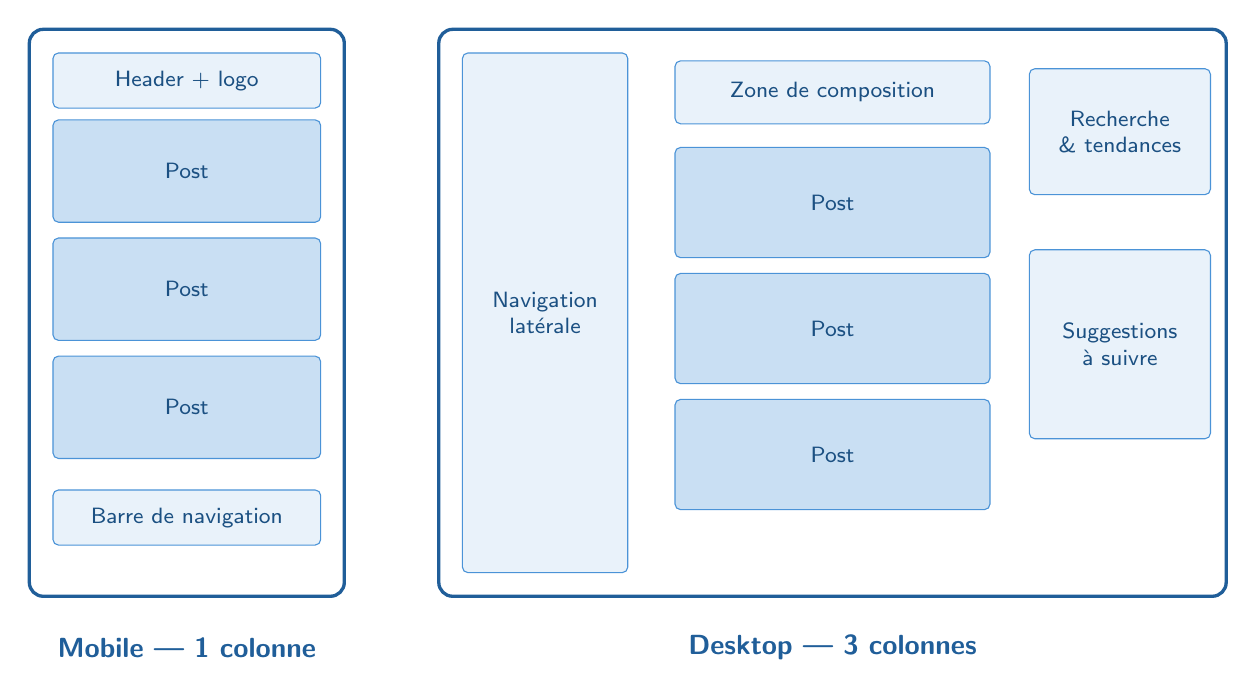
\begin{tikzpicture}[font=\footnotesize\sffamily,
   screen/.style={draw=breezyBlue, very thick, rounded corners=5pt},
   wf/.style={draw=breezyLight, fill=breezyLight!12, rounded corners=2pt,
             align=center, text=breezyBlue!85!black, inner sep=2pt},
   focus/.style={wf, fill=breezyLight!30},
   lbl/.style={align=center, text=breezyBlue, font=\sffamily\bfseries}]

  % ===== Mobile : 1 colonne =====
  \begin{scope}
    \draw[screen] (0,0) rectangle (4,7.2);
    \node[wf, minimum width=3.4cm, minimum height=0.7cm] at (2,6.55) {Header + logo};
    \node[focus, minimum width=3.4cm, minimum height=1.3cm] at (2,5.4) {Post};
    \node[focus, minimum width=3.4cm, minimum height=1.3cm] at (2,3.9) {Post};
    \node[focus, minimum width=3.4cm, minimum height=1.3cm] at (2,2.4) {Post};
    \node[wf, minimum width=3.4cm, minimum height=0.7cm] at (2,1.0) {Barre de navigation};
    \node[lbl] at (2,-0.65) {Mobile --- 1 colonne};
  \end{scope}

  % ===== Desktop : 3 colonnes =====
  \begin{scope}[xshift=5.2cm]
    \draw[screen] (0,0) rectangle (10,7.2);
    % colonne gauche
    \node[wf, text width=1.7cm, minimum width=2.1cm, minimum height=6.6cm]
          at (1.35,3.6) {Navigation latérale};
    % colonne centrale (fil)
    \node[wf, text width=3.6cm, minimum width=4cm, minimum height=0.8cm]
          at (5,6.4) {Zone de composition};
    \node[focus, minimum width=4cm, minimum height=1.4cm] at (5,5.0) {Post};
    \node[focus, minimum width=4cm, minimum height=1.4cm] at (5,3.4) {Post};
    \node[focus, minimum width=4cm, minimum height=1.4cm] at (5,1.8) {Post};
    % colonne droite
    \node[wf, text width=1.9cm, minimum width=2.3cm, minimum height=1.6cm]
          at (8.65,5.9) {Recherche \& tendances};
    \node[wf, text width=1.9cm, minimum width=2.3cm, minimum height=2.4cm]
          at (8.65,3.2) {Suggestions à suivre};
    \node[lbl] at (5,-0.65) {Desktop --- 3 colonnes};
  \end{scope}

\end{tikzpicture}
\caption{Wireframes des dispositions mobile (une colonne, navigation basse) et bureau (trois colonnes : navigation, fil central, tendances).}
\label{fig:wireframe}
\end{figure}

\paragraph{Principes d'ergonomie.} La navigation principale passe d'une barre
inférieure sur mobile à une barre latérale sur bureau ; le fil central reste
l'élément focal ; la colonne de droite (recherche, tendances, suggestions)
n'apparaît qu'à partir des grands écrans. Un thème clair/sombre et un sélecteur de
langue (FR/EN/ES) sont accessibles depuis l'interface.

% =====================================================================
\section{Fonctionnalités principales et mise en œuvre}
% =====================================================================

\subsection{Authentification et gestion des rôles}

L'inscription crée un compte en attente de validation ; la connexion renvoie un
\textbf{jeton JWT} (signé HS256, valable une heure) transmis ensuite dans l'en-tête
\texttt{Authorization: Bearer}. Côté front, le jeton est conservé et injecté
automatiquement dans chaque requête Axios. Le contrôle d'accès (RBAC) est appliqué
côté serveur par un middleware d'authentification, et reflété côté client en
masquant les actions non autorisées (par exemple, le bouton de modération n'est
visible que pour les modérateurs et administrateurs).

\subsection{Publication et fil d'actualité}

La création de post accepte un texte (280 caractères), des tags, et un média
optionnel \textbf{image ou vidéo} : le fichier est d'abord envoyé au service Media,
puis l'URL retournée est attachée au post. Le fil chronologique agrège les posts
des comptes suivis ; un \textit{mapper} dédié transforme le document MongoDB en
modèle d'affichage et résout l'auteur (identifiant → nom).

\subsection{Interactions sociales}

Les likes utilisent une \textbf{mise à jour optimiste} : l'interface bascule
immédiatement puis se recale sur la réponse du serveur (ou annule en cas d'erreur).
Commentaires et réponses imbriquées sont stockés directement dans le document du
post. Le suivi d'un utilisateur met à jour la table relationnelle des abonnements
et déclenche une notification.

\subsection{Notifications et messagerie}

Les notifications (mentions, likes, nouveaux abonnés) sont remontées par un hook
partagé entre l'en-tête et la barre latérale, qui résout les expéditeurs et
formate les libellés. La messagerie privée regroupe les échanges par conversation
et expose le nombre de messages non lus.

\subsection{Modération}

Tout utilisateur peut \textbf{signaler} un contenu ; les signalements alimentent
une file consultable par les modérateurs, qui peuvent les résoudre et, le cas
échéant, \textbf{suspendre ou bannir} un compte. L'accès à l'espace de modération
est protégé côté serveur et masqué côté client aux rôles non habilités.

\subsection{Couche d'intégration front/back}

La liaison entre les deux mondes constitue le cœur de ma contribution. Elle repose
sur :

\begin{itemize}[leftmargin=1.4em]
  \item une \textbf{couche de services Axios} centralisant les appels, la base URL
        de la passerelle et l'injection du jeton ;
  \item une \textbf{enveloppe de réponse standardisée} et des \textit{mappers}
        purs convertissant les modèles back-end en modèles d'affichage ;
  \item la \textbf{passerelle Nginx} réglée pour le CORS, la limitation de débit
        adaptée à une SPA et la diffusion publique des médias ;
  \item un \textbf{déploiement Docker Compose} complet accompagné d'un jeu de
        données de démonstration (utilisateurs liés, posts avec tags, médias et
        notifications) et d'outils web d'inspection des bases (Adminer,
        mongo-express).
\end{itemize}

% =====================================================================
\section{Axes d'amélioration et évolutions}
% =====================================================================

\begin{itemize}[leftmargin=1.4em]
  \item \textbf{Temps réel} — diffusion des notifications et des messages via
        WebSocket plutôt que par interrogation périodique.
  \item \textbf{Recherche avancée} — moteur full-text (posts, utilisateurs, tags)
        et fil de tendances calculé dynamiquement.
  \item \textbf{Observabilité} — journalisation centralisée, métriques et traces
        distribuées sur l'ensemble des microservices.
  \item \textbf{Mise à l'échelle} — orchestration Kubernetes, réplication des bases
        et mise en cache (Redis) des flux les plus consultés.
  \item \textbf{Sécurité} — rafraîchissement des jetons (refresh tokens), HTTPS de
        bout en bout et audit des dépendances automatisé.
  \item \textbf{Qualité} — couverture de tests end-to-end et tests de charge pour
        valider la promesse de scalabilité.
\end{itemize}

% =====================================================================
\section*{Conclusion}
\addcontentsline{toc}{section}{Conclusion}
% =====================================================================

Breezy démontre qu'un réseau social complet peut être bâti sur une architecture
microservices conteneurisée, sécurisée et déployable en une commande, tout en
respectant une exigence de légèreté et de réactivité. Les 23 fonctionnalités
prévues ont été couvertes, de l'authentification à la modération, en passant par
la publication de médias et les interactions sociales.

Au-delà du résultat technique, ce projet a renforcé des compétences clés
d'intégration Full-Stack, de pratiques DevOps (conteneurisation, passerelle API,
déploiement automatisé) et de conduite de projet (organisation Git, priorisation,
coordination d'équipe). Les axes d'évolution identifiés — temps réel,
observabilité et mise à l'échelle — ouvrent des perspectives concrètes pour
transformer ce prototype abouti en service de production.

% ---------------------------------------------------------------------
\newpage
\section*{Sitographie}
\addcontentsline{toc}{section}{Sitographie}

\begin{itemize}[leftmargin=1.4em]
  \item Documentation Next.js — \url{https://nextjs.org/docs}
  \item Documentation Express.js — \url{https://expressjs.com}
  \item Documentation Docker — \url{https://docs.docker.com}
  \item Documentation PostgreSQL / Sequelize — \url{https://sequelize.org}
  \item Documentation MongoDB / Mongoose — \url{https://mongoosejs.com}
  \item Spécification Conventional Commits — \url{https://www.conventionalcommits.org}
\end{itemize}
